\section{Computational Structure}\label{chpt:fmm:sec:computational_structure}

- The data flow is shown in Figure \ref{fig:chpt:fmm:data_flow} for all the operators for a uniform FMM in two dimensions with two levels taken in the hierarchical tree.

- In this section we map this data flow to the available parallelism on shared and distributed memory systems.

- Tree construction

    - bottom up vs top down, complexities of each approach
    - Morton vs Hilbert spatial decompositions
    - ORB as an alternative approach.
    - What are the positives and trade-offs of different spatial encodings? How much do I think it matters?
    - linked list vs linear
        - linear us, pvfmm
        - exafmm-t as an example of linked list variant.

- Interaction list access
    - Originally, based on linked lists - Anderson,
    - Move towards masking techniques, bebendorf GPU and Gumerov, as GPUs became a thing.
    - High degree of success with index pointer based techniques, us, pvfmm and exafmm.

- Runtime, Thread and Data level parallelism
    - threading model
        - tbb/rayon approach on work stealing vs openmp fork-join
    - data level
        - achieved easily if formulated with modern BLAS libraries for critical operators.

- Formulation of translation operators.
    - analytical (unrolled) formulations
        - relies on special functions, multithreading possible but manual
        - can be written as BLAS
    - algebraic
        - BLAS

Ghost data exchange of interaction lists
    - MPI
        - point to point vs collective vs neighbourhood collective
    - Runtime systems
        - BSP (ie MPI) vs task based

    - implications for caching based on granularty of tasks.

How can parallelism best be expressed?

- Unroll the FMM loop
- linearise data access for interaction lists
- ensure that as many key operations as possible can use those implementations with high flop/byte ratio and take advantage of SIMD i.e. open source FFTW/BLAS/LAPACK.

What does this mean in terms of the operators?

- Data dependency at coarsest granularty is over levels, reminiscent of V list cycle in multigrid approaches.
    - Picking this level of granularty gives the greatest flexibility to an implementer to explore options.
    - Furthermore, the P2P and recursive scheme are completely data independent and should be treated as such.

- Ensuring data locality for translations
    - i.e. it's clear that M2M and L2L can be batched over sets of siblings.
        - but can also batch over multiple sets of siblings at each level.

    - the challenge ise the M2L, where the number of accesses is as no order of magnitude larger than M2M and L2L.
    - P2P, standard techniques can be adapted due to natural parallelism over target particles. The challenge is ensuring that SIMD is used appropriately for inverse square roots, and special functions, to fully utilise cache and CPU.
    - tree and admissibility condition should be separated from the data access method
        - i.e. no matter what these are, level-wise data access is always linear over contiguous blocks.

- Parallel model that allows for tunable cache utilisation
    - this means taking advantage of 'free lunches' from open-source software for high performance, relying on BLAS/LAPACK as much as possible as well as FFT if utilised.
        - SIMD special functions, and inverse roots
    - i.e. avoid parallel models where cache coherence could be destroyed for any reason.

- Removing as much as possible into the pre-computation step.
    - i.e. separate out required data into that evaluated at runtime, and that which can be stored and cached.

- Distributed memory
    - Foundational work by Warren and Salmon.
    - naively, due to global data dependency over each level, high levels of the tree are required across the entire domain.
    - BUT the amount of data is actually extreemly small, just the multipole coefficients for long range interactions. The P2P charge data is by definition extremely local, and can be handled effectively even with point to point communication patterns which are simple.
    - modern MPI implementations can do all-reduce style operations in log(P), talk a little about this.
    - MPI 3.0 and above introduce neighbourhood communication
        - Note that, when viewed hierarchically, data exchange is local in terms of morton keys. So maps well to hierarchical neighbourhood collective communication patterns

- Software environment that allows us to mix and match all of the above, and can be a tool for both high performance simulation and algorithmic exploration.

At the end of this we have a skeleton for a high performacne FMM/hierarchical matrix

- Component diagram for high performance abstract FMM:

\begin{figure}[h]
    \includegraphics[width=\textwidth]{fmm_data_flow.png}
    \caption{Data flow for the evaluation of the potentials due to a given set of (red) source particles in the far field of a given set of (blue) target particles, in two dimensions for clarity with a uniform tree of depth two. The source particles in the near field of the target box are shown in grey.}
    \label{fig:chpt:fmm:data_flow}
\end{figure}

- Many past works have alluded to this feature of the FMM, though it is rarely expressed as such explicitly in the literature.

- Early examples include the works of Chandramowlishwaram and co-workers, who develop performance models characterising the kiFMM on various hardwares, and acknowledge the trade-off between the M2L and P2P as the key characteristic for FMM performance, and controlled by the tree depth.

- Deeper trees, synonymous with fewer particles per leaf node, and therefore smaller $U$-lists for P2P, but with more M2L.

- Shallower trees, synonymous with larger P2P and fewer M2L.

- Since then many works have focussed on expressing the data dependencies explicitly, and exposing them to special runtimes. - Proponent of task based runtime systems, as not restricted to specific algorithmic ordering of tasks removes artificial syncs, expose more native concurrency, and shorten critical path. The latter tends to restrict operations to a specific order. DAG-based dynamic runtime engines can remove artifactual synchronizations in the form of subroutine boundaries, remove artifactual orderings in the form of pre-scheduled loops, expose the native concurrency, and shorten the critical path. StarPU, Charm++ and Legion being popular runtimes.

- However as we can see there are remarkably few intra-level synchrnoisations required for the FMM, meaning that the overhead of a runtime system in comparison to ordinary multithreading based appraoches

- The principal drawback of losing this control is that though NUMA aware approaches do exist, it is significantly hardware to control data locality, which i§s critical for performance on modern architectures.

- Furthermore, most critically, the two most expensive operations of the FMM, the P2P and M2L operators, \textit{have no data dependencies} Meaning that there is amply opportunity to develop fully asynchronous implementations of these two operations, and given the optimal SIMD/SIMT structure of the P2P operation the obvious choice of operator to deploy to GPU in a heterogenous implementation.


